\documentclass{article}

\usepackage{amsmath, amsthm, amssymb, amsfonts}
\usepackage{thmtools}
\usepackage{graphicx}
\usepackage{setspace}
\usepackage{geometry}
\usepackage{float}
\usepackage{hyperref}
\usepackage[utf8]{inputenc}
\usepackage[english]{babel}
\usepackage{framed}
\usepackage[dvipsnames]{xcolor}
\usepackage{tcolorbox}

%Define the listing package
\usepackage{listings} %code highlighter
\usepackage{color} %use color
\definecolor{mygreen}{rgb}{0,0.6,0}
\definecolor{mygray}{rgb}{0.5,0.5,0.5}
\definecolor{mymauve}{rgb}{0.58,0,0.82}
 
%Customize a bit the look
\lstset{ %
backgroundcolor=\color{white}, % choose the background color; you must add \usepackage{color} or \usepackage{xcolor}
basicstyle=\footnotesize, % the size of the fonts that are used for the code
breakatwhitespace=false, % sets if automatic breaks should only happen at whitespace
breaklines=true, % sets automatic line breaking
captionpos=b, % sets the caption-position to bottom
commentstyle=\color{mygreen}, % comment style
deletekeywords={...}, % if you want to delete keywords from the given language
escapeinside={\%*}{*)}, % if you want to add LaTeX within your code
extendedchars=true, % lets you use non-ASCII characters; for 8-bits encodings only, does not work with UTF-8
frame=single, % adds a frame around the code
keepspaces=true, % keeps spaces in text, useful for keeping indentation of code (possibly needs columns=flexible)
keywordstyle=\color{blue}, % keyword style
% language=Octave, % the language of the code
morekeywords={*,...}, % if you want to add more keywords to the set
numbers=left, % where to put the line-numbers; possible values are (none, left, right)
numbersep=5pt, % how far the line-numbers are from the code
numberstyle=\tiny\color{mygray}, % the style that is used for the line-numbers
rulecolor=\color{black}, % if not set, the frame-color may be changed on line-breaks within not-black text (e.g. comments (green here))
showspaces=false, % show spaces everywhere adding particular underscores; it overrides 'showstringspaces'
showstringspaces=false, % underline spaces within strings only
showtabs=false, % show tabs within strings adding particular underscores
stepnumber=1, % the step between two line-numbers. If it's 1, each line will be numbered
stringstyle=\color{mymauve}, % string literal style
tabsize=2, % sets default tabsize to 2 spaces
title=\lstname % show the filename of files included with \lstinputlisting; also try caption instead of title
}
%END of listing package%
 
\definecolor{darkgray}{rgb}{.4,.4,.4}
\definecolor{purple}{rgb}{0.65, 0.12, 0.82}
 
%define Javascript language
\lstdefinelanguage{JavaScript}{
keywords={typeof, new, true, false, catch, function, return, null, catch, switch, var, if, in, while, do, else, case, break},
keywordstyle=\color{blue}\bfseries,
ndkeywords={class, export, boolean, throw, implements, import, this},
ndkeywordstyle=\color{darkgray}\bfseries,
identifierstyle=\color{black},
sensitive=false,
comment=[l]{//},
morecomment=[s]{/*}{*/},
commentstyle=\color{purple}\ttfamily,
stringstyle=\color{red}\ttfamily,
morestring=[b]',
morestring=[b]"
}
 
\lstset{
language=JavaScript,
extendedchars=true,
basicstyle=\footnotesize\ttfamily,
showstringspaces=false,
showspaces=false,
numbers=left,
numberstyle=\footnotesize,
numbersep=9pt,
tabsize=2,
breaklines=true,
showtabs=false,
captionpos=b
}

\colorlet{LightGray}{White!90!Periwinkle}
\colorlet{LightOrange}{Orange!15}
\colorlet{LightGreen}{Green!15}

\newcommand{\HRule}[1]{\rule{\linewidth}{#1}}

\NewEnviron{NORMAL}{% 
    \scalebox{2}{$\BODY$} 
} 

\declaretheoremstyle[name=Theorem,]{thmsty}
\declaretheorem[style=thmsty,numberwithin=section]{theorem}
\tcolorboxenvironment{theorem}{colback=LightGray}

\declaretheoremstyle[name=Proposition,]{prosty}
\declaretheorem[style=prosty,numberlike=theorem]{proposition}
\tcolorboxenvironment{proposition}{colback=LightOrange}

\declaretheoremstyle[name=Principle,]{prcpsty}
\declaretheorem[style=prcpsty,numberlike=theorem]{principle}
\tcolorboxenvironment{principle}{colback=LightGreen}

\setstretch{1.2}
\geometry{
    textheight=9in,
    textwidth=5.5in,
    top=1in,
    headheight=12pt,
    headsep=25pt,
    footskip=30pt
}

% ------------------------------------------------------------------------------

\begin{document}

% ------------------------------------------------------------------------------
% Cover Page and ToC
% ------------------------------------------------------------------------------

\title{ \normalsize \textsc{}
		\\ [2.0cm]
		\HRule{1.5pt} \\
		\LARGE \textbf{\uppercase{Cloud Computing}
		\HRule{2.0pt} \\ [0.6cm] \LARGE{Corso A} \vspace*{10\baselineskip}}
		}
\date{\text{Ultima Compilazione - }\today}

\author{\textbf{Autore} \\ 
		Giuseppe Acocella \\
		2024/25\\}

\maketitle
\newpage

\tableofcontents

\newpage

%\begin{figure}[htbp]
    %\center
    %\includegraphics[scale=0.4]{img/classiComplessita2.png}
%\end{figure}

\section{Introduzione}

Il Cloud Computing ha rivoluzionato l'utilizzo dei calcolatori, permettendo di astrarre sull'effettiva implementazione e fornendo numerosi servizi agli utenti. Formalmente il Cloud Computing è un modello che permette di avere accesso alla rete su richiesta di risorse di calcolo configurabili.

\subsection{Servizio vs Bene}
Questo nuovo modo di utilizzare i calcolatori si basa su uno specifico schema, ossia quello del \textbf{servizio} in sostituzione al \textbf{bene} fisico. Un esempio è \textbf{Spotify}: Prima di un applicazione che forniva l'accesso alla musica (\textbf{servizio}) esisteva il \textbf{bene} fisico, ad esempio il vinile. Questo ci permette di astrarre dal concetto di possedimento, lasciando all'utente la possibilità di accedere ad un servizio che non dipende da lui.

\subsection{Service Level Agreement (SLA)}

Ogni rapporto va stabilito formalmente con un contratto. Lo \textbf{SLA} si occupa di questo, permette una formulazione del rapporto tra user e servizio. All'interno si trovano tutti i dettagli su cosa un user deve aspettarsi dal servizio, anche in caso di malfunzionamento ed indisponibilità del servizio stesso.

\subsection{Quality of Matter (QoS)}

La qualità di un servizio offerto dipende fortemente dalle tecnologie su cui si basa, come ad esempio il servizio di hosting. Lo sviluppo dunque di un app ha bisogno di operazioni di \textbf{previsioning} che calcolino le risorse necessarie ad una buona esecuzione del servizio in questione.

\paragraph{Under/Overprevisioning}

Immaginando di stabilire una capacità massima per il nostro servizio:

\begin{enumerate}
    \item \textbf{Underprevisioning}: La capacità massima è inferiore al picco massimo di richiesta al servizio, questo porta a situazioni di stallo e rallentamenti.
    \item \textbf{Overprevisioning}: La capacità massima è inutilmente più grande della media delle richieste, di conseguenza si causa un forte spreco di risorse.
\end{enumerate}

\paragraph{CapEx e Cloud Computing} In passato, per avviare un attività era sempre necessario un primo capitale iniziale, che permettesse il corretto avvio. Molti dei servizi più in voga (IaaS,Paas,SaaS) del cloud computing permettono l'avvio di applicazioni e piccole aziende senza nessuna difficoltà iniziale.

\paragraph{Elasticità e Risk Transfer} Il Cloud Computing offre anche altri vantaggi, risulta infatti molto semplice scalare ad esempio da uno storage di $1Mb$ ad uno di $1Tb$ (\textbf{Elasticità}) dato che l'intera responsabilità della reallocazione viene lasciata alla piattaforma. Lo stesso vale per i backup dei dati, che vengono autonomamente effettuati dalla piattaforma (\textbf{Risk Transfer}).

\newpage

\subsection{Model Service (IaaS, PaaS, SaaS)}

Tutti i servizi definiti prima si basano su un \textbf{modello}, ossia quanto il cloud è "coinvolto", elenchiamo tutti i modelli, nello stack rappresentiamo tutte le \textbf{responsabilità} date all'\textbf{user}:
\vspace*{5px}
\begin{enumerate}
    \item \textbf{IaaS}: Infrastracture as a Service:
    \vspace*{10px}
    \begin{center}
        \begin{tabular}{ |c| } %|c|c|c|%
         \hline
         Sistema Operativo \\
         \hline
         Applicazione \\ 
         \hline
         Dati \\
         \hline
         Impostazione Dati \\
         \hline
        \end{tabular}
    \end{center}
    \vspace*{10px}
    \item \textbf{PaaS}: Platform as a Service:
    \vspace*{10px}
    \begin{center}
        \begin{tabular}{ |c| } %|c|c|c|%
         \hline
         Applicazione \\ 
         \hline
         Dati \\
         \hline
         Impostazione Dati \\
         \hline
        \end{tabular}
    \end{center}
    \vspace*{10px}
    \item \textbf{SaaS}: Software as a Service:
    \vspace*{10px}
    \begin{center}
        \begin{tabular}{ |c| } %|c|c|c|%
         \hline
         Dati \\
         \hline
         Impostazione Dati \\
         \hline
        \end{tabular}
    \end{center}
\end{enumerate}
\vspace*{10px}

\paragraph{Cloud Privato/Ibrido/Pubblico} Ogni azienda nel corso del proprio sviluppo ha la necessità di chiedersi come impostare la propria rete di calcolatori. Illustriamo tre modi:

\begin{enumerate}
    \item \textbf{Cloud Privato}: L'azienda ha la necessità di costruire il proprio data center, prendendosi tutte le responsabilità circostanti come la gestione dei backup, la manutenzione ecc... Questo permette però all'azienda stessa di avere un controllo diretto sui propri server, e di conseguenza dei propri dati.
    \item \textbf{Cloud Pubblico}: L'azienda sceglie di hostare tutti i propri servizi su server offerti da un provider (Amazon, Google, ...). Questo scaricherà tutte le responsabilità sul provider, causando un costo all'azienda.
    \item \textbf{Cloud Ibrido}: L'azienda sceglie di suddividere i propri dati, in modo tale da utilizzare sia server locali sia servizi a pagamento di provider esterni.
\end{enumerate}

\paragraph{Vendor Lock-In} La scelta dell'azienda di utilizzare o meno cloud esterni a pagamento potrebbe portare a difficoltà future di migrazione dato che i provider potrebbero scegliere di "rendere difficile" l'uscita ai clienti. Di conseguenza diventa necessario per le aziende sviluppare un \textbf{exit plan} per una potenziale migrazione.

\newpage

\section{Infrastracture as a Service (IaaS)}

Analizziamo nello specifico l'Infrastruttura come Servizio. Queste si suddividono in due sottocategorie:

\begin{enumerate}
    \item \textbf{Tipo Compute}: Servizio che offre calcolo computazionale virtualizzato, veri e propri calcolatori remoti. Elenchiamo alcune caratteristiche note:
    \begin{enumerate}
        \item Solitamente forniscono \textbf{istanze}, ossia \textbf{server virtuali}.
        \item Spesso utilizzano preset con Windows/Linux.
        \item Gamma di istanze basate su CPU, Memoria, GPU, Storage...
        \item Istanze a pagamento secondo i criteri \textbf{on demand}\footnote{Pagamento proporzionato all'utilizzo.} oppure \textbf{istanza spot}\footnote{Pagamento fisso}.
    \end{enumerate}
    Un esempio di questo tipo di servizio è \textbf{Amazon EC2}.
    \item \textbf{Tipo Storage}: Servizio che offre spazio di archiviazione. Elenchiamo alcune caratteristiche note:
    \begin{enumerate}
        \item \textbf{Backup} automatici.
        \item \textbf{Versioning} di dati offerto di default.
        \item \textbf{Classi} di memorizzazione in base alla \textbf{frequenza} d'\textbf{accesso}.
        \item Configurazioni predefinite di \textbf{sicurezza} e \textbf{cifratura}.
    \end{enumerate}
\end{enumerate}

\subsection{Hypervisors}

Gli Hypervisors permettono la gestione di ambienti virtuali sulla stessa macchina fisica. Illustriamo lo stack dei due possibili tipi di Hypervisors:

\begin{enumerate}
    \item \textbf{Tipo 1}: Stack caratterizzato dall'assenza del \textbf{Host OS}:
    \begin{center}
        \begin{tabular}{ |c| } %|c|c|c|%
        \hline
        App A \:\: \vline \:\: App B \\
        \hline
        Bins/Libs \:  \vline \:  Bins/Libs \\
        \hline
        Guest OS \:  \vline \:  Guest OS \\        
         \hline
         Hypervisor \\ 
         \hline
         Hardware \\
         \hline
        \end{tabular}
    \end{center}

    \item \textbf{Tipo 1}: Stack caratterizzato dalla presenza del \textbf{Host OS}:
    \begin{center}
        \begin{tabular}{ |c| } %|c|c|c|%
        \hline
        App A \:\: \vline \:\: App B \\
        \hline
        Bins/Libs \:  \vline \:  Bins/Libs \\
        \hline
        Guest OS \:  \vline \:  Guest OS \\        
         \hline
         Hypervisor \\ 
         \hline
         Host OS \\
         \hline
         Hardware \\
         \hline
        \end{tabular}
    \end{center}
\end{enumerate}

Solitamente il tipo 1 è utilizzato nei data center, mentre il tipo 2 nei personal computer che hanno la necessità di virtualizzare per qualche specifico motivo.

\newpage

\subsection{Identity and Access Managment (IaM)}

L'\textbf{IaM} gestisce l'accesso sicuro ai servizi, e si suddivide in due specifiche operazioni:

\begin{enumerate}
    \item \textbf{Autenticazione}: $User_1$ viene confrontato ad un attesa identità di $User_1$, \\ confrontando quindi identità corrente ad una virtuale.
    \item \textbf{Autorizzazione}: Dopo aver autenticato $User_1$ è necessario stabilire quali permessi possieda.
\end{enumerate}

L'\textbf{IaM} è detta eventually consistent perchè spesso i sistemi dipendono da transazioni distribuite che causano \textbf{inconsistenza temporanea}, questa va risolta successivamente, quindi non si riesce ad affermare che il sistema sia sempre \textbf{consistente}.

\section{Containers e Virtualizzazione}

Vogliamo generare degli "ambienti virtuali" come nel caso degli hypervisors senza però portarsi dietro un vero e proprio \textbf{Guest OS}. Di conseguenza immaginiamo uno schema del genere:

\vspace*{5px}

\begin{center}
        \begin{tabular}{ |c| } %|c|c|c|%
        \hline
        App A \:\: \vline \:\: App B \\
        \hline
        Bins/Libs \:  \vline \:  Bins/Libs \\
        \hline
         Container Manager \\ 
         \hline
         Host OS \\
         \hline
         Hardware \\
         \hline
        \end{tabular}
    \end{center}

\vspace*{15px}

La \textbf{virtualizzazione} di \textbf{ambiente} è un processo che esiste da molto tempo, ma lo standard degli ultimi anni è stato definito da Docker. 

\textbf{Docker} è una piattaforma che ci permette di lanciare applicazioni in ambienti isolati, questo genera una \textbf{completa portabilità} di un applicazione da macchina a macchina grazie alla virtualizzazione di tutte le dipendenze.

\vspace*{15px}


\paragraph{Confronto con Hypervisors} Il \textbf{Docker Engine} dunque gestisce i container sulla 

macchina fisica come l'\textbf{Hypervisor} gestisce le varie macchine virtuali sulla macchina fisica.

\vspace*{15px}

\paragraph{Volume} Quando un applicazione richiede la persistenza dei dati anche dopo l'arresto risulta necessario l'utilizzo di un volume, ossia un "disco d'archiviazione virtuale" compatibile nativamente con i container. Questi possono essere utilizzati per rendere condivise risorse tra i container.

\newpage

\subsection{Dockerfile, Immagine, Container}

Entriamo nello specifico, descrivendo le fasi di costruzioni di un container:

\begin{enumerate}
    \item \textbf{Dockerfile}: File di testo che segue una specifica sintassi e permette al \textbf{Docker Engine} di interpretarlo ed eseguire le istruzioni al suo interno che terminano producendo un immagine.
    \item \textbf{Registry}: Riferimento ad un immagine online, una sorta di repository, solitamente ottenibile da \textbf{Dockerhub}.
    \item \textbf{Image}: Oggetto \textbf{eseguibile} dal Docker Engine, permette di costruire un container sulla base dell'immagine data.
    \item \textbf{Container}: Effettivo ambiente virtuale generato sulla macchina. Questo può essere mandato in esecuzione permettendo alle applicazioni al suo interno di lavorare in ambienti protetti ed isolati.
\end{enumerate}

\begin{figure}[htbp]
    \center
    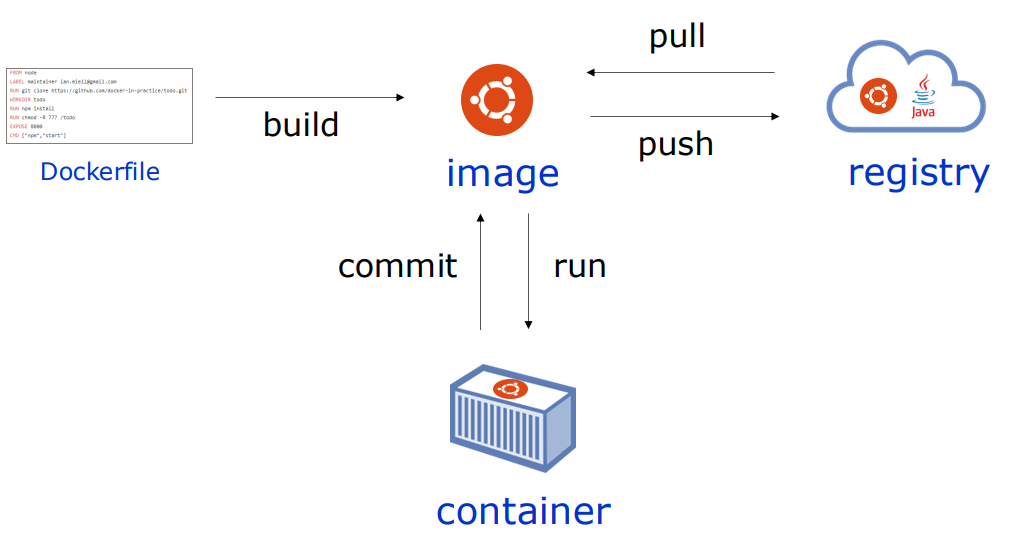
\includegraphics[scale=0.35]{img/howWorksDocker.png}
\end{figure}

\subsection{Docker Compose, Docker Swarm e Mapping Porte}

\vspace*{10px}

\paragraph{Docker Compose} Grazie ad un file di configurazione in formato $yaml \:(.yml)$ permette la coordinazione di più microservizi su container diversi. In questo modo si permette la comunicazione tra microservizi grazie alla \textbf{rete overlay} settata dal Docker Compose.

\paragraph{Docker Swarm} Servizio di supporto offerto da Docker che permette varie semplificazioni:

\begin{enumerate}
    \item Rete di microservizi diversi divisa in nodi \textbf{worker} e nodi \textbf{manager}.
    \item Riorganizzazione del lavoro tra i nodi in caso di fail di specifici nodi.
    \item Reboot automatico (detto Self Healing) in caso di fail dei microservizi sui container.
\end{enumerate}

\paragraph{Mapping di Porte dei Container} A causa della virtualizzazione si crea inconsistenza sulla gestione delle porte, infatti i container faranno riferimento a delle \textbf{porte virtuali} non realmente esistenti sulla macchina, anche essendo "rappresentate dallo stesso numero". Di conseguenza diventa compito di \textbf{Docker} e di chi gestisce le applicazioni gestire il map delle \textbf{porte virtuali} su \textbf{porte reali} della \textbf{macchina fisica}.

\newpage

\section{Function as a Service (FaaS)}

Questo tipo di modello porta il livello d'astrazione quasi al massimo, dando la possibilità all'user di inserire il proprio codice in una e vera \textbf{textbox} ed eseguirlo direttamente. In questo modo si deresponsabilizza del tutto l'utente dalla configurazione e gestione di ambienti/macchine virtuali. Si basa sulla \textbf{Event Driven Programming}, ossia programmazione guidata dall'avvenimento di specifici eventi. Gli ambienti forniti dai provider di (FaaS) sono compatibili con la maggior parte dei linguaggi e le relative librerie.

\paragraph{Trigger e API Gateway} Spesso queste funzioni si espongono all'esterno grazie a dei \textbf{trigger}, come ad esempio un \textbf{API Gateway} che ci permette di effettuare delle \textbf{GET/POST} in direzione della funzione stessa.

\subsection{AWS Lambda e Definizione di Serverless} AWS offre il proprio servizio di (FaaS), anche il più utilizzato al momento sul mercato. Questo servizio è \textbf{AWS Lambda} e permette di caricare funzioni ed interagire con esse con l'impostazione dei trigger definiti prima. La lontananza tra l'user e la configurazione del server su cui sta lavorando caratterizza la definizione di \textbf{serverless}. \textbf{Ovviamente l'user sta utilizzando un server}, ma lo sta facendo in maniera "\textbf{implicita}".

\paragraph{AWS Step Function} Lo sviluppo su AWS Lambda non si limita a singole funzioni atomiche, ma si estende anche a veri e propri sistemi di microfunzioni che interagiscono tra loro secondo uno specifico diagramma di flusso, realizzando intere applicazioni. Le Step Function si basano dunque sulla combinazione di $\lambda$funzioni che seguono un workflow specifico. Il cosiddetto servizio di orchestrazione permette di parallelizzare, mettere in serie, in loop ecc... una quantità arbitraria di funzioni.

\paragraph{Pricing di AWS Lambda} Una caratteristica fondamentale di questo servizio è quella di definire il proprio costo in base all'utilizzo delle chiamate alla funzione lambda in questione. Questo comporta costi modici anche sull'ordine dei milioni di chiamate. Chiaramente viene però effettuato uno \textbf{scaling} anche in base alle risorse utilizzate (memoria e tempo di computazione) dalla chiamata alla funzione.

\subsubsection{Pesante Vendor Lock In delle FaaS}

Immaginiamo di aver costruito un intera applicazione grazie alla composizione di funzioni lambda. Se per qualche motivo dovesse risultare necessario cambiare provider del servizio (FaaS) allora avremmo un gran problema. Questo perchè i \textbf{trigger} delle funzioni della nostra applicazione \textbf{sono proprietari}. Di conseguenza non è impossibile migrare verso un nuovo provider ma risulta \textbf{molto difficile}, dovendo modificare il codice sorgente dell'applicazione. Dunque ogni tipo di semplificazione sulla configurazione e sulla manutenzione del ambiente la pago in potenziale libertà di movimento.

\newpage

\section{Platform as a Service (PaaS)}

Questo modello basato sulla piattaforma come servizio deresponsabilizza ancora di più l'utente
rispetto all'infrastruttura come servizio, l'user infatti non dovrà occuparsi della \textbf{gestione dell'ambiente}
e questo modello risulta anche facilmente adattabile a nuove tecnologie. Nello specifico l'user non sarà più
il responsabile della gestione del \textbf{Setup}, dello \textbf{Scale} e del \textbf{Managment}.
Solitamente l'IaaS viene utilizzato in contesti di sviluppo, debug, testing o deployment.

\paragraph{Differenze tra PaaS e IaaS} Spesso il confine tra questi due tipi di modelli non è ben definito, infatti molti provider forniscono contemporaneamente sia PaaS sia Iaas.
Formalmente però il PaaS è più ad alto livello, liberando l'user da ancora più responsabilità. Un esempio di piattaforma come servizio può essere l'utilizzo di un IDE online. Solitamente nei PaaS ci
vengono fornite direttamente le piattaforme d'utilizzo dell'user e non l'accesso diretto alla macchina host.

\paragraph{Add-On e Lock In dei PaaS} Una delle migliori funzionalità di questo modello è la presenza di Add Ons
che offrono la possibilità di aggiungere estensioni quasi in modalità "drag and drop". Questo tipo di aggiunte però
lega l'applicazione al corrente provider di (PaaS), dato che tutti i plug in aggiunti sono proprietari. In tale modo si definisce un
tipo intrinseco di \textbf{lock in} del provider sull'applicazione.



\subsection{Heroku} Servizio cloud (PaaS) basato su containerizzazione di ambienti. La caratteristica di questi container è la loro facile scalabilità.
I container di questo servizio sono denominati \textbf{dynos}, e la loro gestione automatica genera grande
scalabilità del servizio.

\paragraph{Scalabilità dei Dynos} L'user non dovrà mai occuparsi della gestione manuale delle dynos, ma
queste verranno scalate automaticamente in base alle richieste effettuate al servizio hostato sulle varie dynos.
Sono quindi dei container basati su Linux autogestiti sotto il punto di vista dello scaling.

\paragraph{Build/Run Time} Durante il tempo di build, avendo a disposizione il codice sorgente da deployare e tutta la lista di dipendenze, si compone un \textbf{Procfile} che
contiene il comando da eseguire all'avvio. L'esecuzione del procfile è detta \textbf{build} e produce un oggetto detto \textbf{slug}.
Il tempo di run invece acquisendo uno \textbf{slug} permette la costruzione di uno stack e "l'engine" saprà quante dynos dedicare all'esecuzione dello slug in questione.
La grande scalabilità si basa anche sullo schema simil "produttore/consumatore" utilizzato spesso tra i vari tipi di dynos.
\newpage

\end{document}